\newthought{\textbf{Salsabila Irmanda - 2020903430048 - TRKJ 3B}}

\newday{\textbf{1 - 2 Desember 2022} - Instalasi dan Konfigurasi Hadoop}
\begin{enumerate}
\item Kendala dan Solusi\\
\begin{enumerate}
\item Saat melakukan percobaan instalasi hadoop terdapat kendala yaitu saat melakukan extrak file hadoop, solusi yang digunakan yaitu memberikan ukuran ruang lebih besar saat membuat os ubuntu
\item Melakukan konfigurasi apache hadoop pratikan mengalami kendala pada perintah format HDFS. solusi yang digunakan yaitu mengecek lagi file - file konfigurasi hadoop hingga tidak ada lagi kesalahan
\end{enumerate}
% jelaskan kendala dan penyebab yang dialami saat mengikuti praktikum serta solusi atau langkah-langkah yang telah dilakukan

\item Kesimpulan \\
Adapun kesimpulan yang diperoleh yaitu tahap instalasi dan konfigurasi hadoop telah berhasil. untuk mengecek hadoop service dengan perintah jps.
% berikan kesimpulan dari praktikum yang telah dikerjkan
\begin{figure}[!ht]
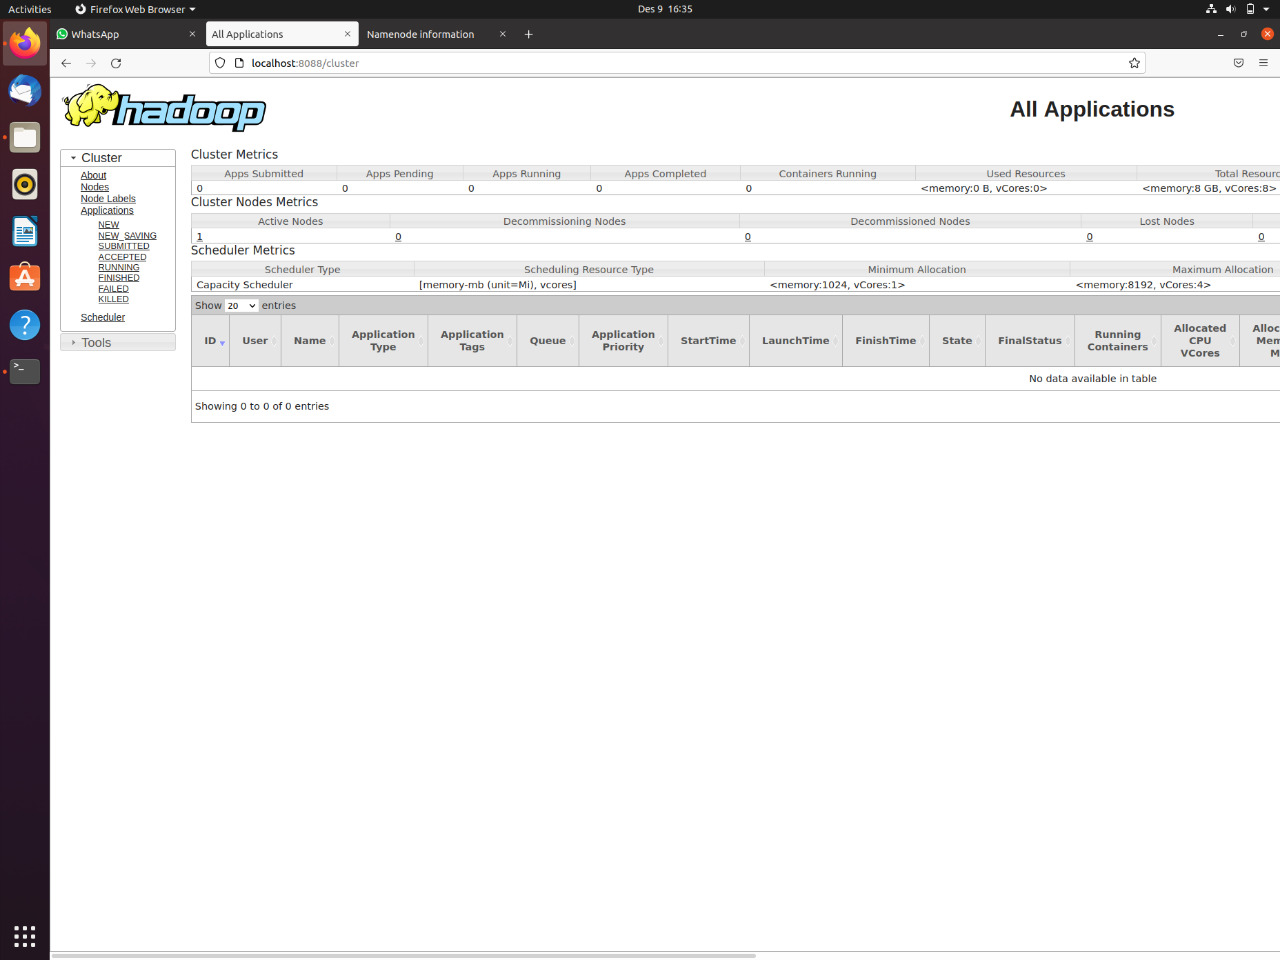
\includegraphics[width=.8\textwidth]{SalsabilaIrmanda/1}
\caption{localhost:8088}
\label{gam:perkuliahan-22-09}
\end{figure}

\newpage
\begin{figure}[!ht]
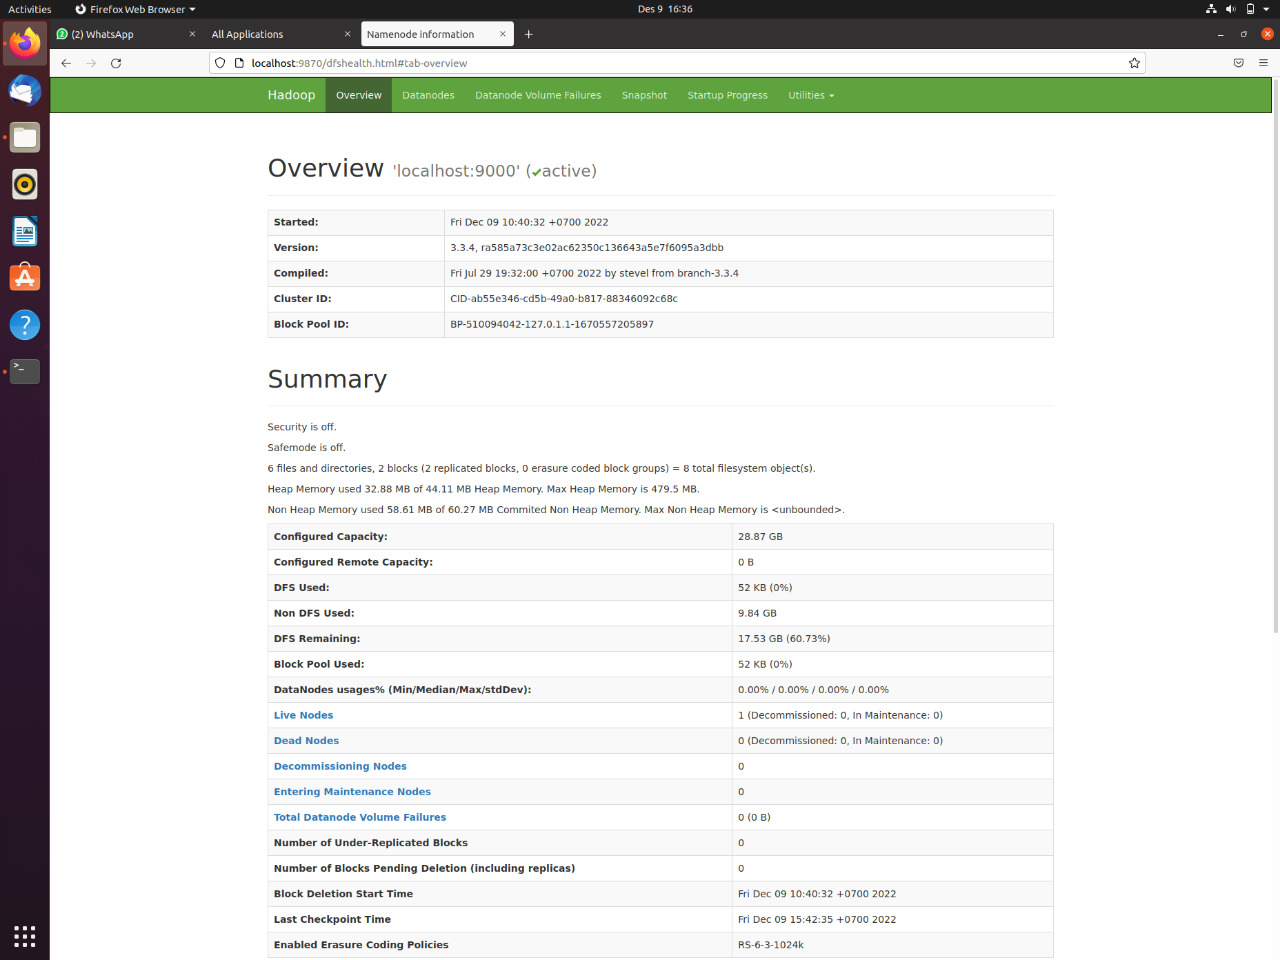
\includegraphics[width=\textwidth]{SalsabilaIrmanda/2}
\caption{localhost:9870}
\label{gam:perkuliahan-22-09}
\end{figure}
\end{enumerate}


\newday{\textbf{8 Desember 2022} - WordCount bawaan Hadoop}
\begin{enumerate}
\item Kendala dan Solusi \\
Saat melakukan percobaan program Word Count Hadoop tidak mengalami kendala. 
% jelaskan kendala dan penyebab yang dialami saat mengikuti praktikum serta solusi atau langkah-langkah yang telah dilakukan
\item Kesimpulan \\
setelah melanjutkan percobaan dan mengikuti semua langkah hingga selesai pratikan berhasil menjalankan ouput program wordcount bawaan hadoop. 

% berikan kesimpulan dari praktikum yang telah dikerjkan
\begin{figure}[!ht]
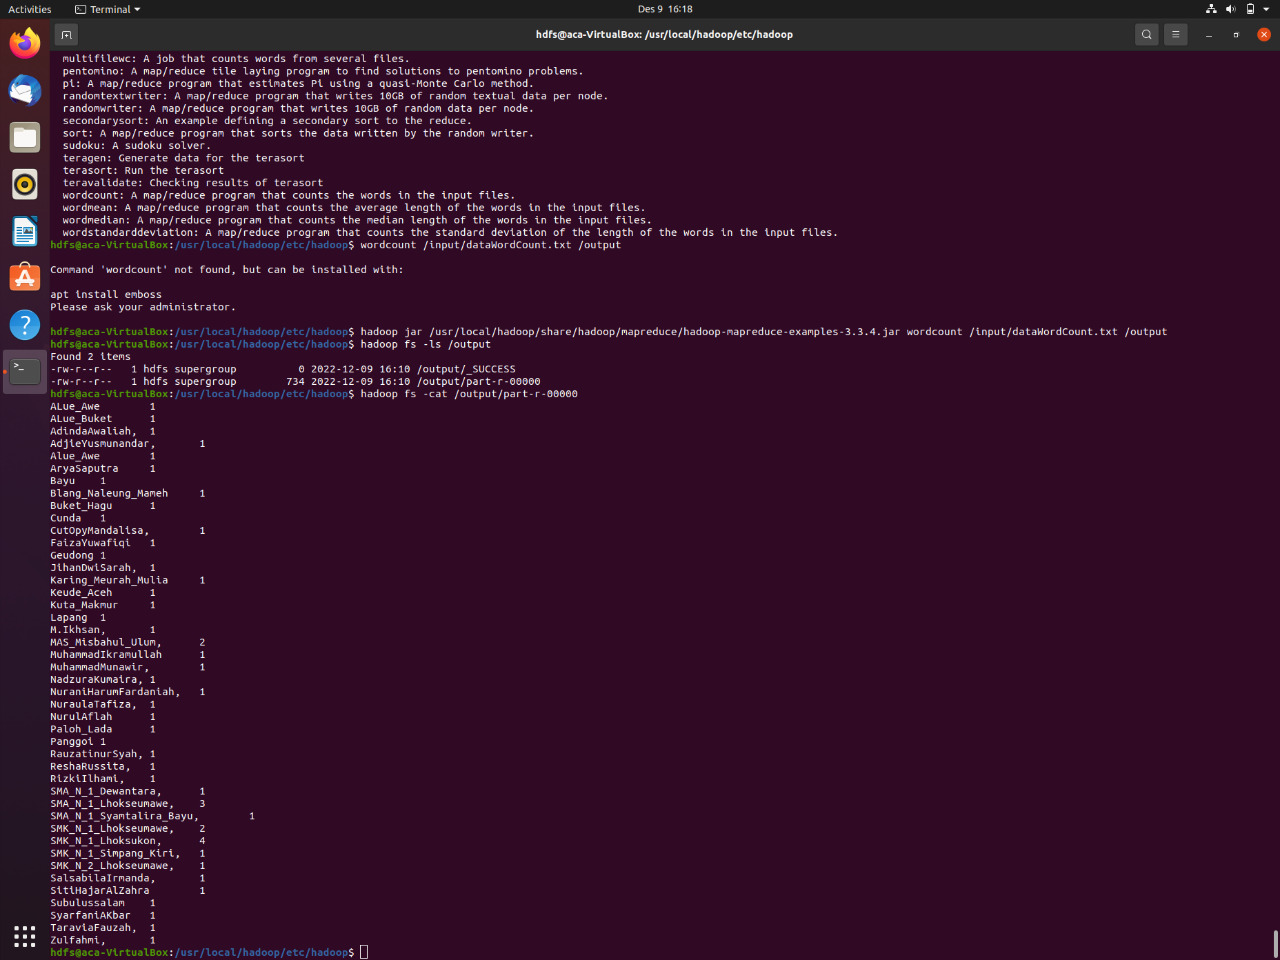
\includegraphics[width=\textwidth]{SalsabilaIrmanda/langkah6&7}
\caption{Hasil perhitungan Wordcount bawaan hadoop berdasarkan output}
\label{gam:perkuliahan-08-12}
\end{figure}
\end{enumerate}

\newday{\textbf{9 Desember 2022} - WordCount dengan Java}
\begin{enumerate}
\item Kendala dan Solusi \\
Terdapat kendala saat melakukan cek hasil pada program wordcount dengan java, solusi nya yaitu harus menjalankan hadoop service. 
% jelaskan kendala dan penyebab yang dialami saat mengikuti praktikum serta solusi atau langkah-langkah yang telah dilakukan

\item Kesimpulan \\
percobaan yang telah dilakukan yaitu melakukan proses membuat program, menyiapkan data, meng-compile program hingga menjalankan program dan berhasil menampilkan hasilnya.
% berikan kesimpulan dari praktikum yang telah dikerjkan

\begin{figure}[!ht]
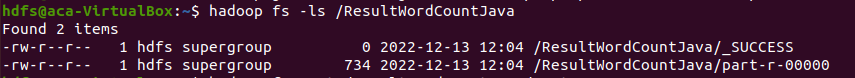
\includegraphics[width=\textwidth]{SalsabilaIrmanda/langkah9}
\caption{hasil program wordcount java 9}
\label{gam:hasil}
\end{figure}

\begin{figure}[!ht]
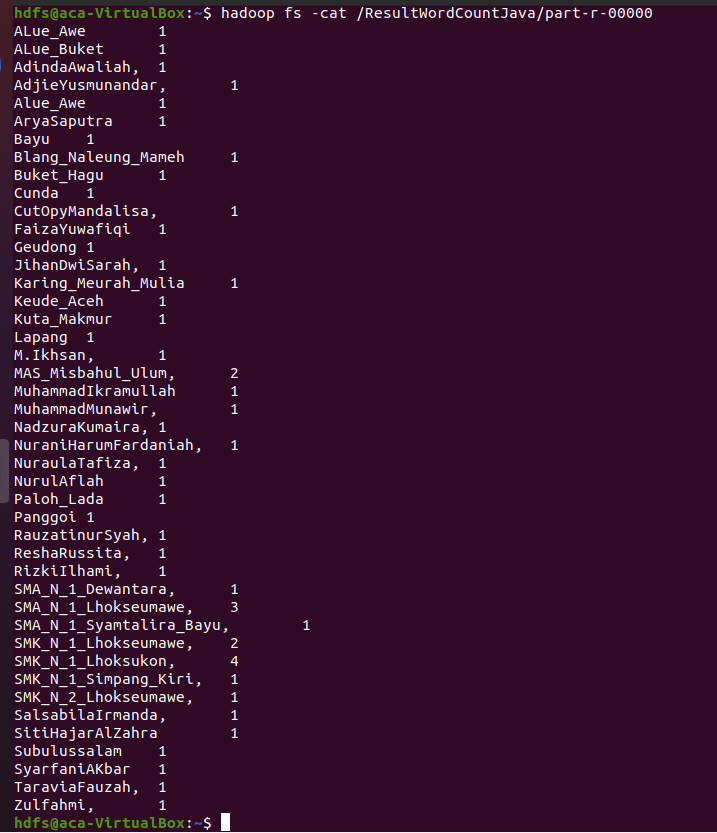
\includegraphics[width=\textwidth]{SalsabilaIrmanda/langkah10}
\caption{hasil program wordcount java 10}
\label{gam:hasil}
\end{figure}
\end{enumerate}

\newday{\textbf{15 Desember 2022}}
\begin{enumerate}
\item Kendala dan Solusi
% jelaskan kendala dan penyebab yang dialami saat mengikuti praktikum serta solusi atau langkah-langkah yang telah dilakukan

\item Kesimpulan
% berikan kesimpulan dari praktikum yang telah dikerjkan

\end{enumerate}